\chapter{Testergebnisse}

Um sicherzustellen, dass die versprochene Funktionalit�t vorhanden ist, sollen die Tests aus dem Pflichtenheft, welche noch g�ltig sind, durchgef�hrt werden. Aus zeitlichen Gr�nden wurden nur die im Pflichtenheft notierten und immer noch relevanten Tests durchgef�hrt.

\begin{table}[H]
	\centering
	\begin{tabularx}{\textwidth}{| l | X |}
		\hline
		\multicolumn{2}{| l |}{\textbf{T1 Indexierung des Medienordners}} \\ \hline
		\textbf{Szenario} & Der Benutzer f�gt seine ``Eigene Musik'' zur Library hinzu und startet den Indexer. \\\hline
		\textbf{Erwartet} & Alle MP3 Dateien mit korrekten ID3-Tags werden laut Log erkannt. \\\hline
		\textbf{Ist} & Die Indexierung wird fehlerfrei durchgef�hrt und die Statistiken stimmen (Abbildung \ref{fig:indexer_output}).
		
		Im Falle der Abbildung wurden acht vollst�ndig getaggte MP3-Dateien und eine nicht getaggte Ogg Vorbis-Datei im Library-Ordner platziert - das Ergebnis stimmt damit �berein.
		\\\hline
		\textbf{Fazit} & Erf�llt \\
		\hline
	\end{tabularx}
\end{table}

\begin{figure}[h]
	\centering
	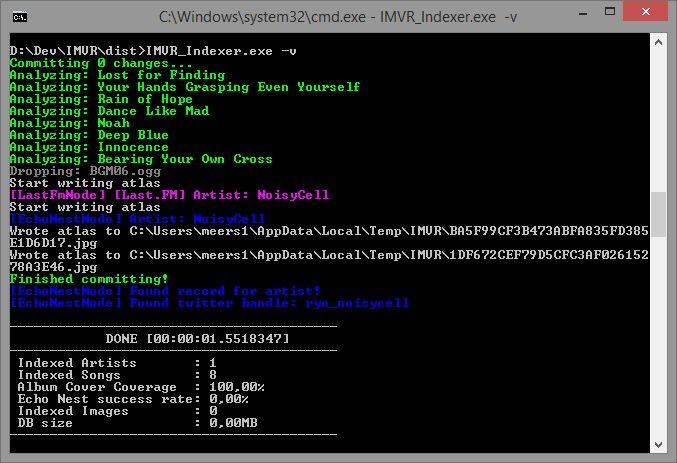
\includegraphics[width=0.6\linewidth]{bilder/indexer_output}
	\caption{Ausf�hrlicher Output des Indexers}
	\label{fig:indexer_output}
\end{figure}

\begin{table}[H]
	\centering
	\begin{tabularx}{\textwidth}{| l | X |}
		\hline
		\multicolumn{2}{| l |}{\textbf{T2 Anzeigen der Gruppierungen}} \\ \hline
		\textbf{Szenario} & Der Benutzer �ffnet die Applikation und wechselt in den Musikmodus. \\\hline
		\textbf{Erwartet} & Die soeben hinzugef�gte Musik erscheint alphabetisch geordnet. \\\hline
		\textbf{Ist} & Der Artist (NoisyCell) wurde korrekt unter ``N'' eingeordnet (Abbildung \ref{fig:noisycell})
		\\\hline
		\textbf{Fazit} & Erf�llt \\
		\hline
	\end{tabularx}
\end{table}

\begin{figure}[h]
	\centering
	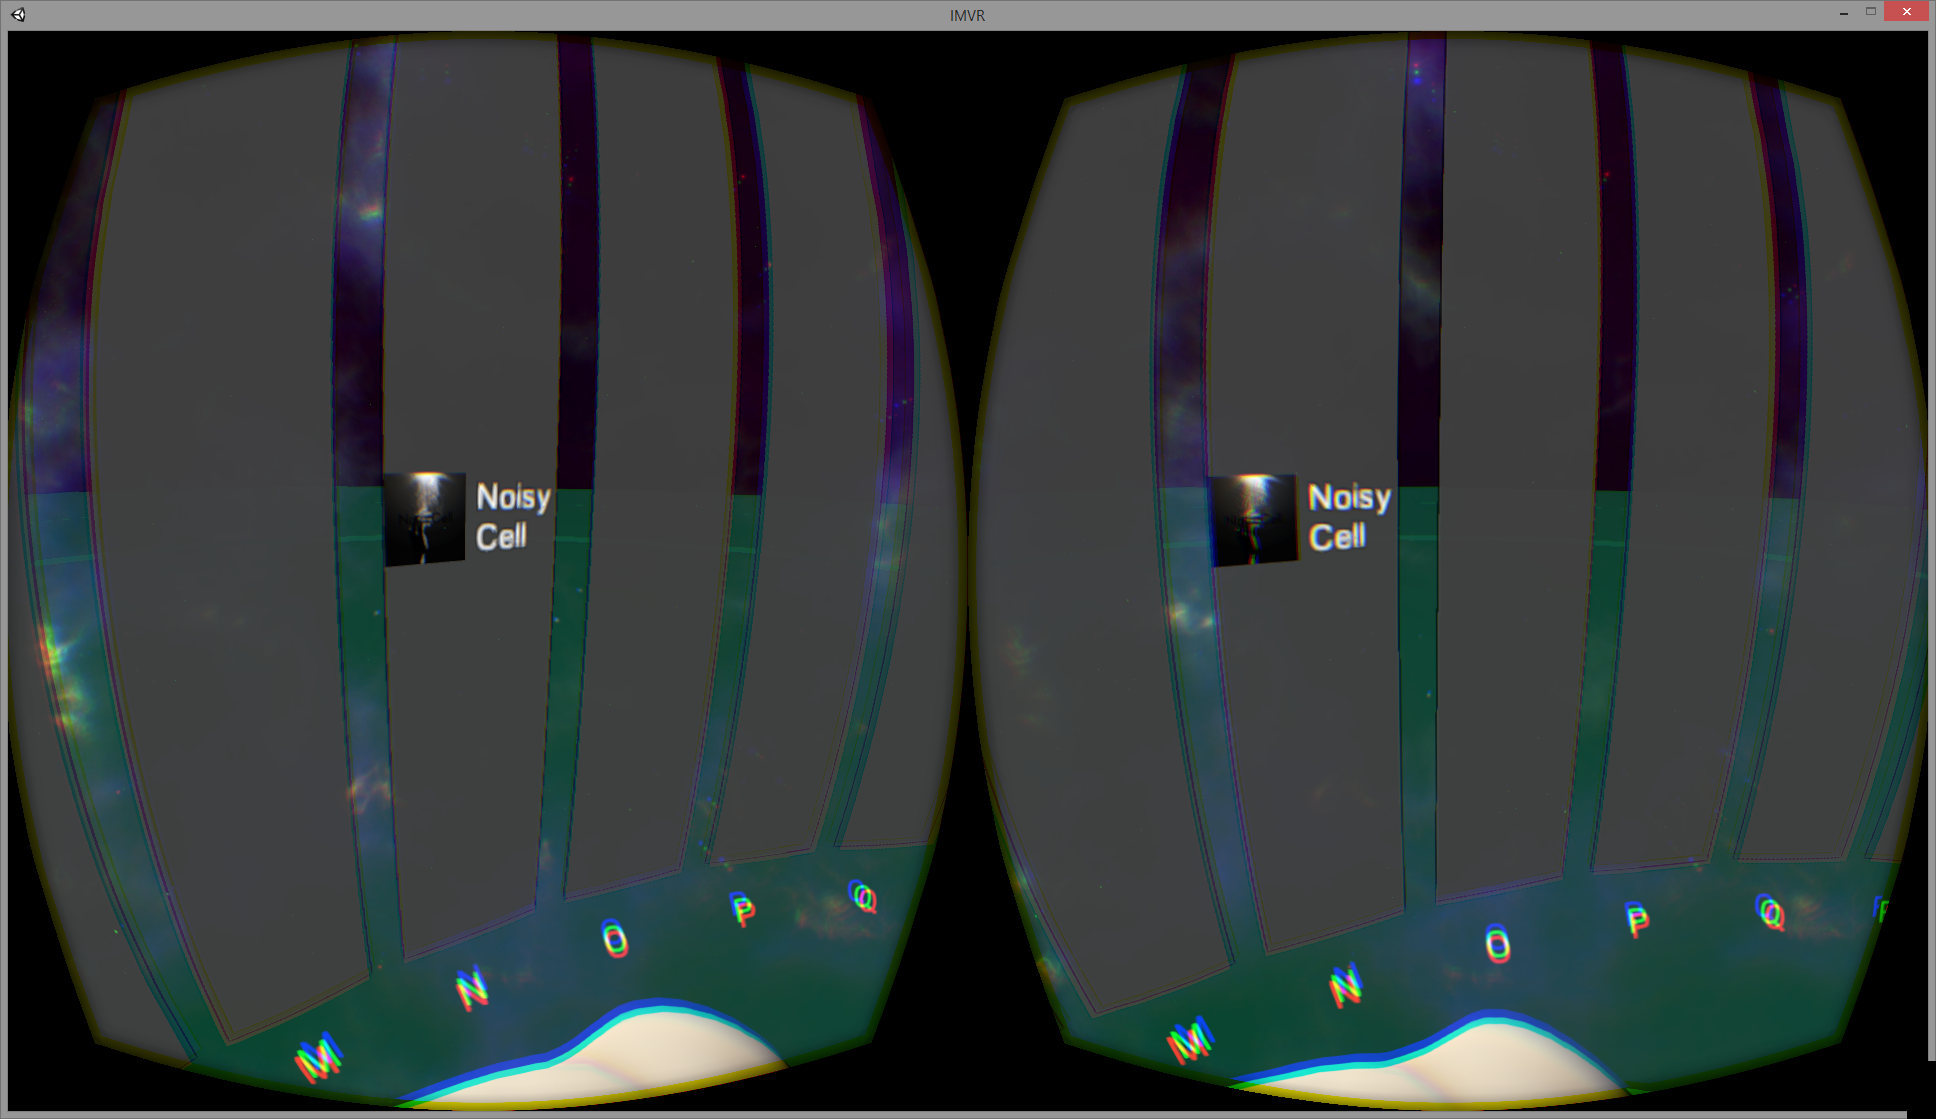
\includegraphics[width=0.9\linewidth]{bilder/noisycell}
	\caption{Screenshot des Resultats von Test T2}
	\label{fig:noisycell}
\end{figure}

\begin{table}[H]
	\centering
	\begin{tabularx}{\textwidth}{| l | X |}
		\hline
		\multicolumn{2}{| l |}{\textbf{T3 Beendigung der Applikation}} \\ \hline
		\textbf{Szenario} & Der Benutzer �ffnet das Hauptmen� und beendet die Applikation. \\\hline
		\textbf{Erwartet} & Die Applikation fragt einmal nach und beendet dann. \\\hline
		\textbf{Ist} & Ein gehaltener Blick auf die entsprechende Bodenplatte reicht zum Beenden. Es wird allerdings nicht nachgefragt.
		\\\hline
		\textbf{Fazit} & Teilweise erf�llt \\
		\hline
	\end{tabularx}
\end{table}